\documentclass[tikz, border=10pt]{standalone}
\usepackage[siunitx, american]{circuitikz}

\begin{document}
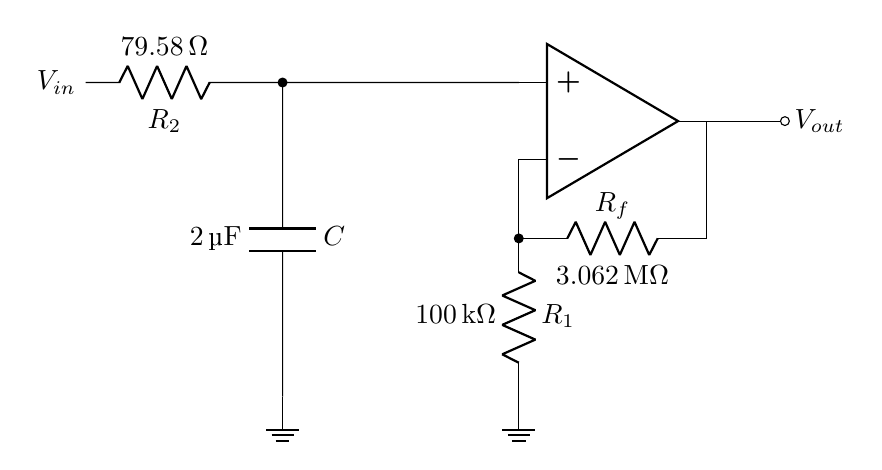
\begin{tikzpicture}
    % Op Amp
    \node[op amp, yscale=-1] (opamp) at (5,0) {};
    
    % RC Input Stage
    \draw (opamp.+) -- ++(-3,0) coordinate (vc) -- ++(-0.5,0)
          to[R, l=$R_2$, a=\SI{79.58}{\ohm}] ++(-2,0) node[short, -o] {} node[left] {$V_{in}$};
    \draw (vc) to[C, l=$C$, a=\SI{2}{\micro\farad}, *-] (vc |- 0,-3.5) node[ground]{};
    
    % Feedback Network
    \draw (opamp.-) -- ++(0,-1) coordinate (vm);
    \draw (vm) to[R, l=$R_1$, a=\SI{100}{k\ohm}] (vm |- 0,-3.5) node[ground]{};
    \draw (vm) to[R, l=$R_f$, a=\SI{3.062}{M\ohm}, *-] (vm -| opamp.out) -- (opamp.out);
          
    % Output
    \draw (opamp.out) to[short, -o] ++(1,0) node[right] {$V_{out}$};

\end{tikzpicture}
\end{document}
